\documentclass{beamer}
% \usetheme{metropolis}
% \usetheme{Warsaw}
\usepackage[utf8]{inputenc}

\usepackage[absolute,overlay]{textpos}
\usepackage{graphicx}

\beamertemplatenavigationsymbolsempty

\usepackage{courier}

\title{\texttt{Computação Quântica}}
\institute{IM-UFRJ}
\date{19 de novembro de 2019}

\author{Pedro Maciel Xavier}

\newcommand{\ket}[1]{\left|#1\right\rangle}
\newcommand{\bra}[1]{\left\langle|#1\right|}

\newcommand{\braket}[2]{\left\langle#1|#2\right\rangle}

\newcommand{\ketbra}[2]{\left|#1\right\rangle\left\langle#2\right|}

\newcommand{\comich}[1]{
	\bgroup
	\setbeamercolor{background canvas}{bg=white}
	\begin{frame}[plain]{}
		\begin{center}
			\begin{figure}
				\includegraphics[height=\textheight]{#1}
			\end{figure}
		\end{center}
	\end{frame}
	\egroup
}

\newcommand{\comic}[1]{\comich{#1}}

\newcommand{\comicw}[1]{
	\bgroup
	\setbeamercolor{background canvas}{bg=white}
	\begin{frame}[plain]{}
	\begin{center}
		\begin{figure}
			\includegraphics[width=\textwidth]{#1}
		\end{figure}
	\end{center}
\end{frame}
\egroup
}

\newcommand{\comicfinal}[1]{
	\bgroup
	\usebackgroundtemplate{\includegraphics[width=\paperwidth]{#1}}
	\begin{frame}[plain]{}

	\end{frame}
	\egroup
}



\begin{document}

	\begin{frame}{Título}
		%\titlepage
	\end{frame}

	\begin{frame}
		\tableofcontents
	\end{frame}

	\comich{bits0.pdf}
	\comich{bits1.pdf}
	\comich{bits2.pdf}
	\comich{bits3.pdf}
	\comich{bits4.pdf}
	\comicfinal{blue-screen.pdf}

	\section{Computação Digital}
	
	\begin{frame}{\textit{bits}}
	
	\vspace{-90pt}
	
	Sobre os \textit{bits}:
		\begin{itemize}
			\item Eles moram em $\mathbb{Z}_2$
			\item Formam vetores em $\mathbb{Z}_2^n$, onde cada $\vec{a} = (a_1, a_2, \dots, a_n) \in \mathbb{Z}_2^n$ representa um valor entre $00...0 = 0$ e $11...1 = 2^n-1$
			\item Realizamos operações \textit{Booleanas} com eles: $\neg$, $\wedge$, $\vee$, $\oplus$.
		\end{itemize}
		\begin{textblock*}{3cm}(2cm, 4cm) % {block width} (coords)
			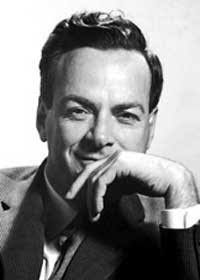
\includegraphics[width=3cm]{feynman.jpg}
			George Boole\\
			{\centering\small 1918 - 1988}
		\end{textblock*}
		
		\begin{textblock*}{3cm}(6cm, 4cm) % {block width} (coords)
			\begin{align*}
				\neg : \mathbb{Z}_2 &\to \mathbb{Z}_2\\
				a &\to \bar{a} = (1 - a)
			\end{align*}
		\end{textblock*}	
	\end{frame}
	
	\begin{frame}
		\begin{itemize}
		\item
		\end{itemize}
	\end{frame}
	
	\comich{first-transistor.pdf}	

	\frame%
	{
		\title{Portas Lógicas}
	}

	\frame%
	{
		\frametitle{Arquitetura de Von Neuman}
		
		\begin{textblock*}{4cm}(2cm, 2cm) % {block width} (coords)
			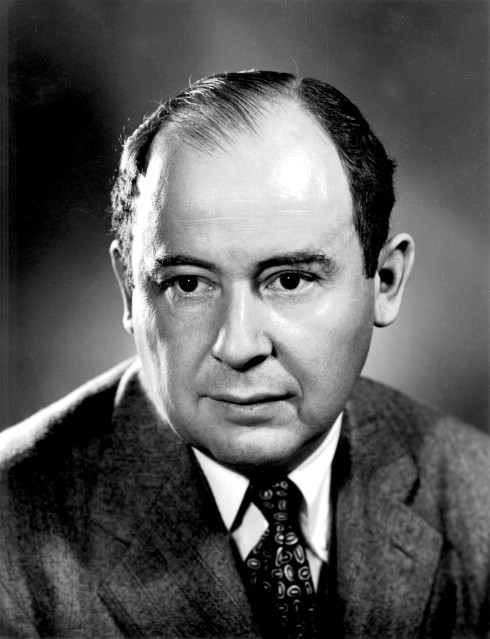
\includegraphics[width=4cm]{von-neuman.jpg}
			John Von Neuman\\
			{\centering\small 1903 - 1957}
		\end{textblock*}
	}

	\begin{frame}{Fenômenos Quânticos}
		\begin{textblock*}{4cm}(2cm, 2cm) % {block width} (coords)
			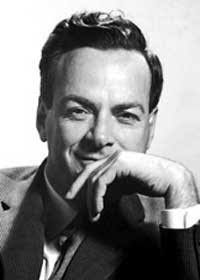
\includegraphics[width=4cm]{feynman.jpg}
			Richard Feynman\\
			{\centering\small 1918 - 1988}
		\end{textblock*}		
	\end{frame}

	\section{Exprimentos}
	\frame{Experimentos}

	\subsection{Algoritmos Quânticos}
	
	\frame%
	{
		\frametitle{Algoritmo de Grover}
		
		\begin{textblock*}{4cm}(2cm, 2.5cm) % {block width} (coords)
			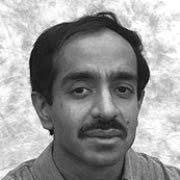
\includegraphics[width=4cm]{grover.jpg}
			Lov Grover\\
			{\centering\small Ex-Bell Labs}
		\end{textblock*}		
	}

	\begin{frame}{Algoritmo de Shor}
		
		\begin{textblock*}{4cm}(2cm, 2.5cm) % {block width} (coords)
			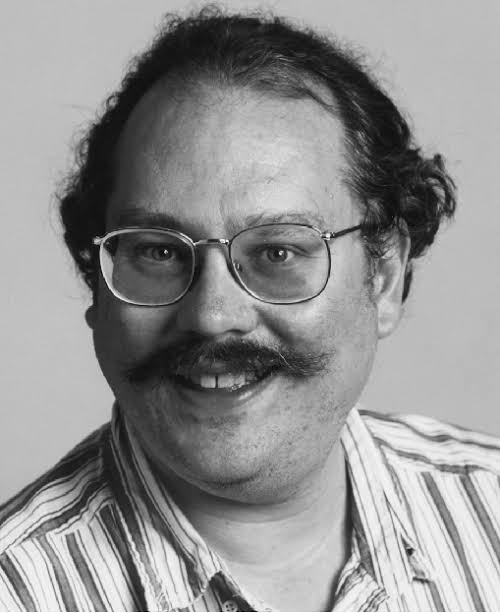
\includegraphics[width=4cm]{shor.jpg}
			Peter Shor\\
			{\centering\small MIT}
		\end{textblock*}		
	\end{frame}
	
	
	\comicw{quantum-teleportation.pdf}
	
	\begin{frame}{Teletransporte Quântico}
	
	\end{frame}
	
	
	\begin{frame}
		\thebibliography{99}
		\bibitem{field:2018} \textbf{Introduction to topological quantum computation with non-Abelian anyons}, FIELD, B. \& SIMULA, T., School of Physics and Astronomy, Monash University, Victoria 3800, Australia.
	\end{frame}
\end{document}